\noindent
\begin{tabular}{cc}
\begin{minipage}{0.60\textwidth}
%\sectionIf{\flagSect}{\taitol{Esercizio}}
\begin{exercise}[Legge di Archimede]
Si consideri, sulla superficie terrestre, un recipiente di diametro $D=2 \ m$ e profondit\`a $H=
3\  m$
contenente acqua ($\rho = 998\ kg / m^3$). Al suo interno \`e inserita una sfera di raggio $a=0.2\, m$
e densit\`a pari a $\rho_s=842.06\ kg / m^3$.
Determinare in modo univoco la posizione assunta dalla sfera nel
liquido. Tale posizione varia se invece che sulla terra ci si trova
sulla luna?\\ 
($h=0.3\  m$, non varia sulla luna.)
\end{exercise}
\end{minipage}
&
\begin{minipage}{0.35\textwidth}
   \begin{center}
   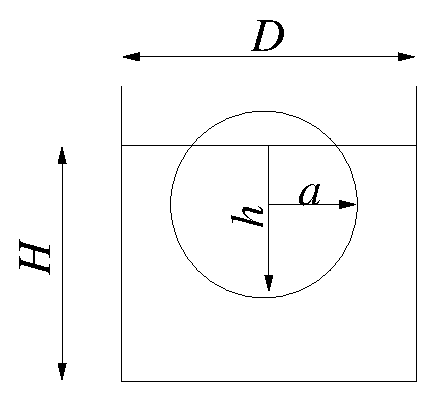
\includegraphics[width=0.90\textwidth]{./fig/recipientesfera.eps}
   \end{center}
\end{minipage}
\end{tabular}

%\vspace{1.0cm}
%\textbf{Soluzione.}

\sol

\partone
Legge di Archimede. Condizione di equilibrio. Calcolo del volume di solidi  (integrali di volume). Adimensionalizzazione. Soluzione di semplici equazioni non lineari per via grafica (studio di funzione) e/o numerica.

\parttwo
Per svolgere l'esercizio bisogna calcolare la condizione di equilibrio del corpo, soggetto alla propria forza peso e alla forza che il fluido esercita su di esso (legge di Archimede). Nell'equazione di equilibrio, l'incognita $h$ compare nella formula del volume immerso nel fluido. L'equazione di equilibrio è un'equazione non lineare in $h$, da risolvere per via grafica
o numerica.
\begin{itemize}
  \item Scrittura dell'equazione di equilibrio del corpo soggetto al proprio peso e alla forza esercitata su di esso dal fluido, diretta verso
  l'alto e pari al peso del volume del fluido spostato (legge di Archimede).
    \begin{equation}\label{eqn:equil_archimede}
      \rho_s V_s g = \rho V_c g \quad\Rightarrow\quad \rho_s V_s = \rho V_c
    \end{equation}
    
  \textit{Osservazione.} Si trova subito la risposta all'ultimo quesito: poiché $g$ non compare nell'equazione di equilibrio, la condizione di equilibrio sulla Luna è uguale a quella che si ha sulla Terra.
  \item Calcolo del volume della sfera e della calotta sferica:

   \begin{itemize}    
     \item Volume della sfera: $V_s = \frac{4}{3}\pi a^3$ %(vergogna se non lo si sa subito!!!)
    
     \item Volume della calotta sferica: $V_c = \pi h^2 (a - \frac{h}{3})$
     
      (per credere, verificare casi limite: $h=0$, $h=a$, $h=2a$; alla fine dell'esercizio è riportato il calcolo, tramite un integrale di volume)
    \end{itemize}
    
  \item Le formule per i volumi $V_c$ e $V_s$ sono inserite nell'eq.
   \ref{eqn:equil_archimede}. L'equazione viene semplificata e scritta in forma adimensionale, introducendo la variabile $x=\frac{h}{a}$, per mettere in evidenza il parametro che governa il problema, cioè il rapporto di densità $\rho_s/\rho$. L'equazione di terzo grado in x viene risolta, considerando i limiti fisici del problema ($0 \le x \le 2$):
    \begin{equation}
      \rho \pi h^2 \Big(a-\frac{h}{3}\Big) = \rho_s \frac{4}{3}\pi a^3  \quad\Rightarrow\quad
      \frac{3}{4} x^2 \Big(1 - \frac{x}{3}\Big) = \frac{\rho_s}{\rho}
    \end{equation}
  Alcuni metodi per risolvere equazioni non lineari possono essere ad esempio:
  \begin{itemize}
    \item metodi iterativi. Ad esempio metodo di Newton
    \begin{center}
\begin{verbatim}
x          res 
1.0000    -3.437475e-01  
1.4583    -2.406993e-02  
1.4990    -5.841602e-04  
1.5000    -4.027539e-07  
1.5000    -1.924017e-13
\end{verbatim}
\end{center}
    
    \item metodo grafico (educativo: per problemi più complicati, prima di calcolare le soluzioni con metodi
    numerici, è bene avere un'idea di cosa si sta cercando).
    Si cercano le intersezioni delle funzioni $f_1(x) = \frac{3}{4} x^2 \Big(1 - \frac{x}{3}\Big)$ e $f_2(x) = \frac{\rho_s}{\rho}$.
  
\begin{center}
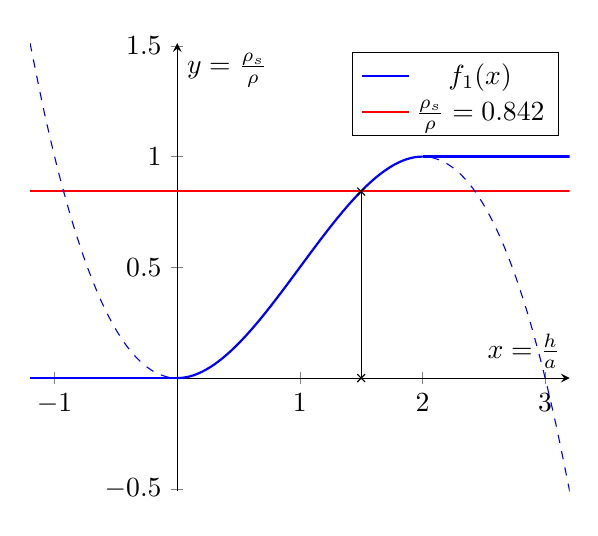
\begin{tikzpicture}
\begin{axis}[axis lines=middle, domain=-1.2:3.2, xlabel={$x=\frac{h}{a}$}, ylabel={$y=\frac{\rho_s}{\rho}$}]
\addplot
[domain=0:2,samples=40,smooth,thick,blue]
{3/4 * (x^2 * (1-x/3))};
\addplot
[domain=-1.2:3.2,samples=40,smooth,thick,red]
{842.06/998};
\addplot
[domain=-1.2:3.2,samples=40,smooth,dashed,blue]
{3/4 * (x^2 * (1-x/3))};
\addplot
[domain= 2.0:3.2,samples=40,smooth,thick,blue]
{1.0};
\addplot
[domain=-1.2:0.0,samples=40,smooth,thick,blue]
{0.0};
\addplot[color=black,mark=x] coordinates{
         (1.50, 0)
         (1.50, 0.842)};
\legend{$f_1(x)$,$\frac{\rho_s}{\rho}=0.842$}
\end{axis}
\end{tikzpicture}
\end{center}
    
  \end{itemize}
  
\end{itemize}

\textit{Osservazione.} Per valori di $\frac{\rho_s}{\rho}$ compresi tra
 0 e 1, esiste una e una sola soluzione fisica del problema.
% Come giustamente \textbf{suggerito da un vostro compagno},
 Per i valori di desità
 ``estremi'' $\rho_s = 0$ (la sfera non pesa niente), $\rho_s = \rho_f$ (la sfera
 ha la stessa densità del fluido), esistono infinite soluzioni:
 ad esempio, nel caso di $\rho_s = \rho_f$ la posizione di equilibrio è indipendente
 dalla profondità alla quale è posta la sfera. Nel grafico, la funzione
 $f_1(x)$ rappresenta il volume immerso della sfera (diviso il volume totale
 della sfera stessa) al variare della 
 distanza $h$ del punto più basso dal pelo libero: questa deve quindi
 essere rappresentata, come in figura, nulla per valori di $x<0$ (sfera
 completamente fuori dall'acqua), con il ramo di cubica per $0<x<2$
 (sfera parzialmente immersa), uguale a $1$ per $x>2$ (sfera completamente
 immersa). La funzione $f_1(x)$ può quindi essere definita a tratti:
 \begin{equation}
  f_1(x) = 
 \begin{cases}
   0 &    x < 0 \\
   \frac{3}{4} x^2 \Big(1 - \frac{x}{3}\Big) &    0 \leq x \leq 2 \\
   1 &   x > 2 \\
 \end{cases}
 \end{equation}
\vspace{0.2cm}

\textit{Discussione dei risultati.} Quando diminuisce la denistà relativa
 del solido, la linea rossa si abbassa e la soluzione $x=\frac{h}{a}$
 diminuisce (la sfera ha una porzione maggiore al di fuori dall'acqua).
 Esiste una e una sola soluzione che abbia senso fisico, fino a quando
 la densità relativa è compresa tra 0 e 1: non ha senso considerare valori
 negativi (la densità è una quantità positiva), mentre per valori di
 $\frac{\rho_s}{\rho}$ maggiori di 1 non può esistere una condizione
 di equilibrio statico (la sfera affonda...).


\newpage
\textbf{Calcolo volume cupola sferica.} 
\'E comodo svolgere il calcolo in coordinate cilindriche $(r,\theta,z)$.
Il volume $V_{im}$ della parte immersa è uguale a 
\begin{equation}
\begin{aligned}
V_{im} = \iiint_{V_{im}} dV & = \int_{\theta=0}^{2\pi} \int_{z=-a}^{l} \int_{r=0}^{\sqrt{a^2-z^2}} dV \\
                & = \int_{\theta=0}^{2\pi} \int_{z=-a}^{l} \int_{r=0}^{\sqrt{a^2-z^2}} r dr dz d\theta \\
                & = 2\pi \int_{z=-a}^{l} \frac{a^2-z^2}{2} dz \\
                & = \frac{\pi}{3} [2 a^3 + 3 a^2 l - l^3]
\end{aligned}
\end{equation}

Definendo $h = R+l$ come la quota immersa della sfera, si ottiene:
\begin{equation}
V_{im} = \pi h^2 \displaystyle \left( a - \frac{h}{3} \right)
\end{equation}


